\documentclass[dvipdfmx,aspectratio=169]{beamer}
\usepackage{pxjahyper}							%しおりの文字化けを防ぐ
\renewcommand{\kanjifamilydefault}{\gtdefault}	%日本語フォントをゴシックに
\usepackage{graphics}							%各種画像の張り込み
\usepackage{amsmath,amssymb,mathtools}					%標準数式表現を拡大する
\usepackage{ulem}
\usepackage{ascmac,fancybox}
\usetheme[
	block=fill,
	progressbar=foot,
	numbering=fraction,
	subsectionpage=progressbar
]{Metropolis}
\usefonttheme{professionalfonts}

\usepackage{here}
\usepackage{booktabs}
\usepackage{hyperref}

\usepackage{tikz}
\usetikzlibrary{positioning}
\usepackage{color}

\newcommand{\highlight}[2][yellow]{\tikz[baseline=(x.base)]{\node[rectangle,rounded corners,fill=#1!10](x){#2};}}
\newcommand{\highlightcap}[3][yellow]{\tikz[baseline=(x.base)]{\node[rectangle,rounded corners,fill=#1!10](x){#2} node[below of=x, color=#1]{#3};}}

\hypersetup{
	colorlinks=true,
	linkcolor=black,
	urlcolor=cyan
}

\title{ディープラーニングの仕組みを知ろう!}
\subtitle{第3回 人工知能勉強会}
\author{Shion MORISHITA}
\institute{}
\date{\today}

\subject{\LaTeX{}+Beamer}
\begin{document}
	%タイトル
	\begin{frame}[plain]
	    \maketitle
	\end{frame}
		
	\begin{frame}[shrink]{目次}
		\vspace{1em}
		\tableofcontents
	\end{frame}
	
	\section{はじめに}
	\begin{frame}{目的}
		\begin{itemize}
			\item 誤差逆伝播法について、その計算方法を理解する
			\item 誤差逆伝播法が勾配降下法の問題点を解決することを理解する
		\end{itemize}
	\end{frame}
	
	\section{勾配降下法の復習}
	\begin{frame}{勾配降下法のイメージ}
		\underline{ボールが転がる方向に向かってパラメータ(ここでは$ x $)を更新}
		
		\begin{figure}
			\centering
			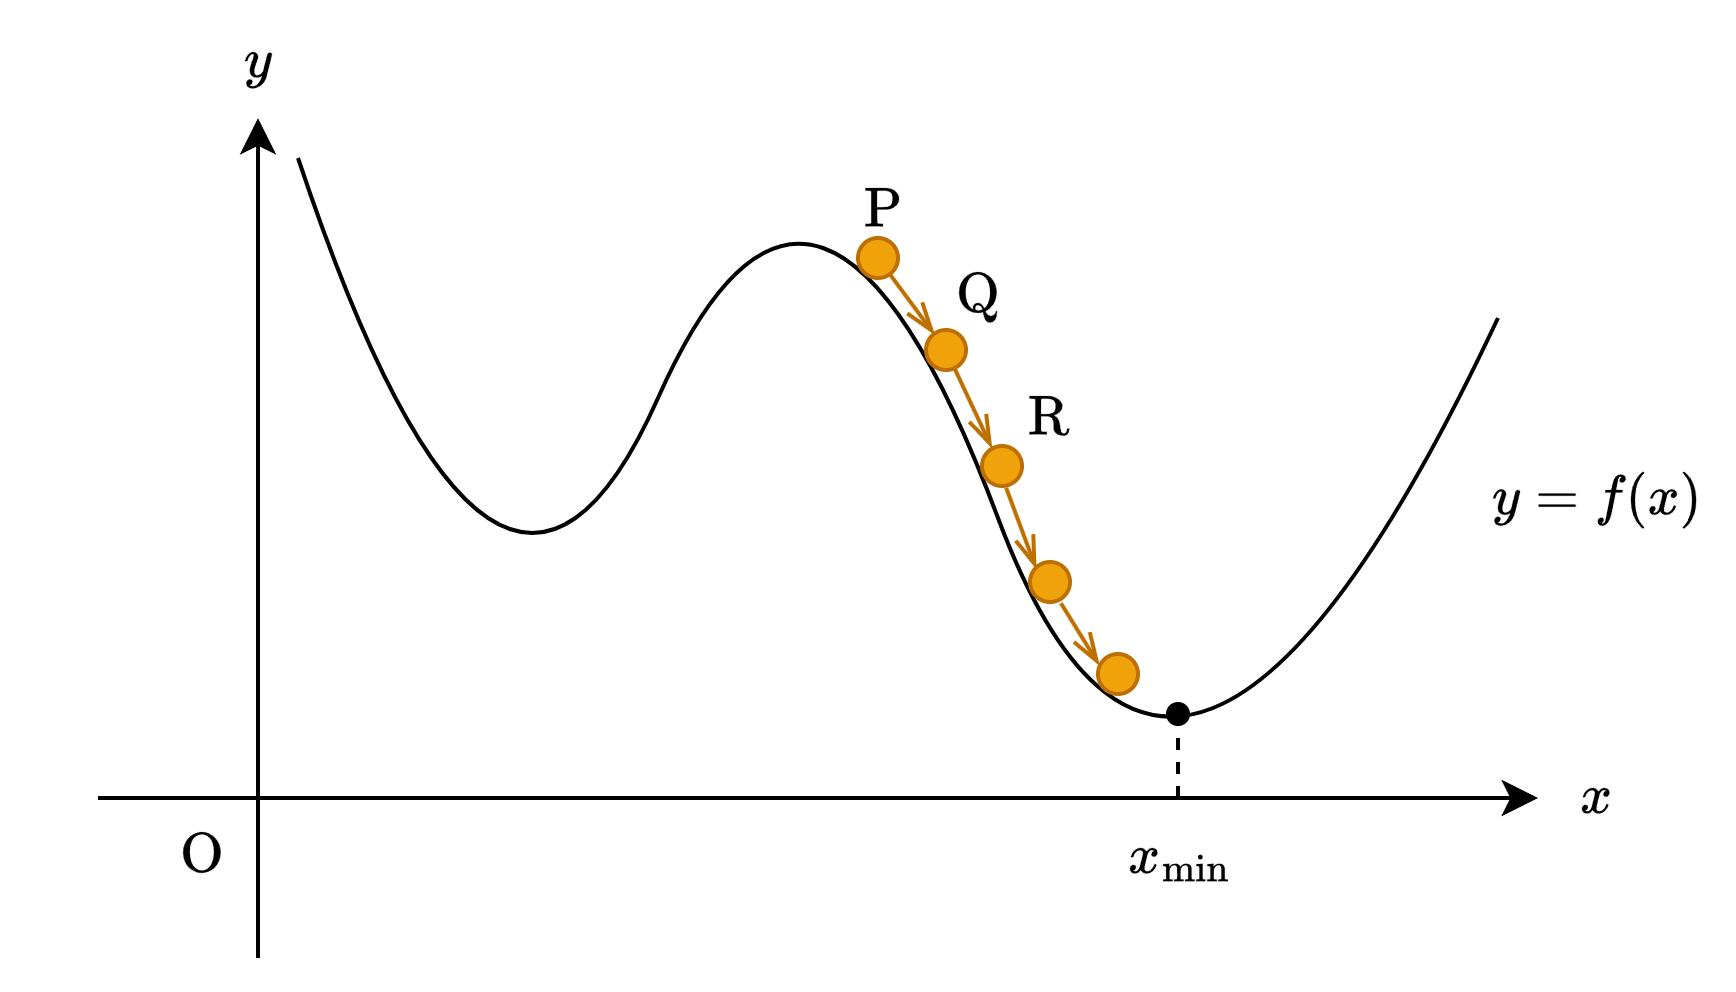
\includegraphics[width=0.7\linewidth]{img/image-of-a-ball-rolling-down-a-slope}
		\end{figure}
		
	\end{frame}
	\begin{frame}{ニューラルネットワークのパラメータ}
		\underline{$ w^2_{11}, \dots, w^3_{11}, \dots, b^2_1, \dots, b^3_1, \dots $がパラメータ}
		\begin{figure}
			\centering
			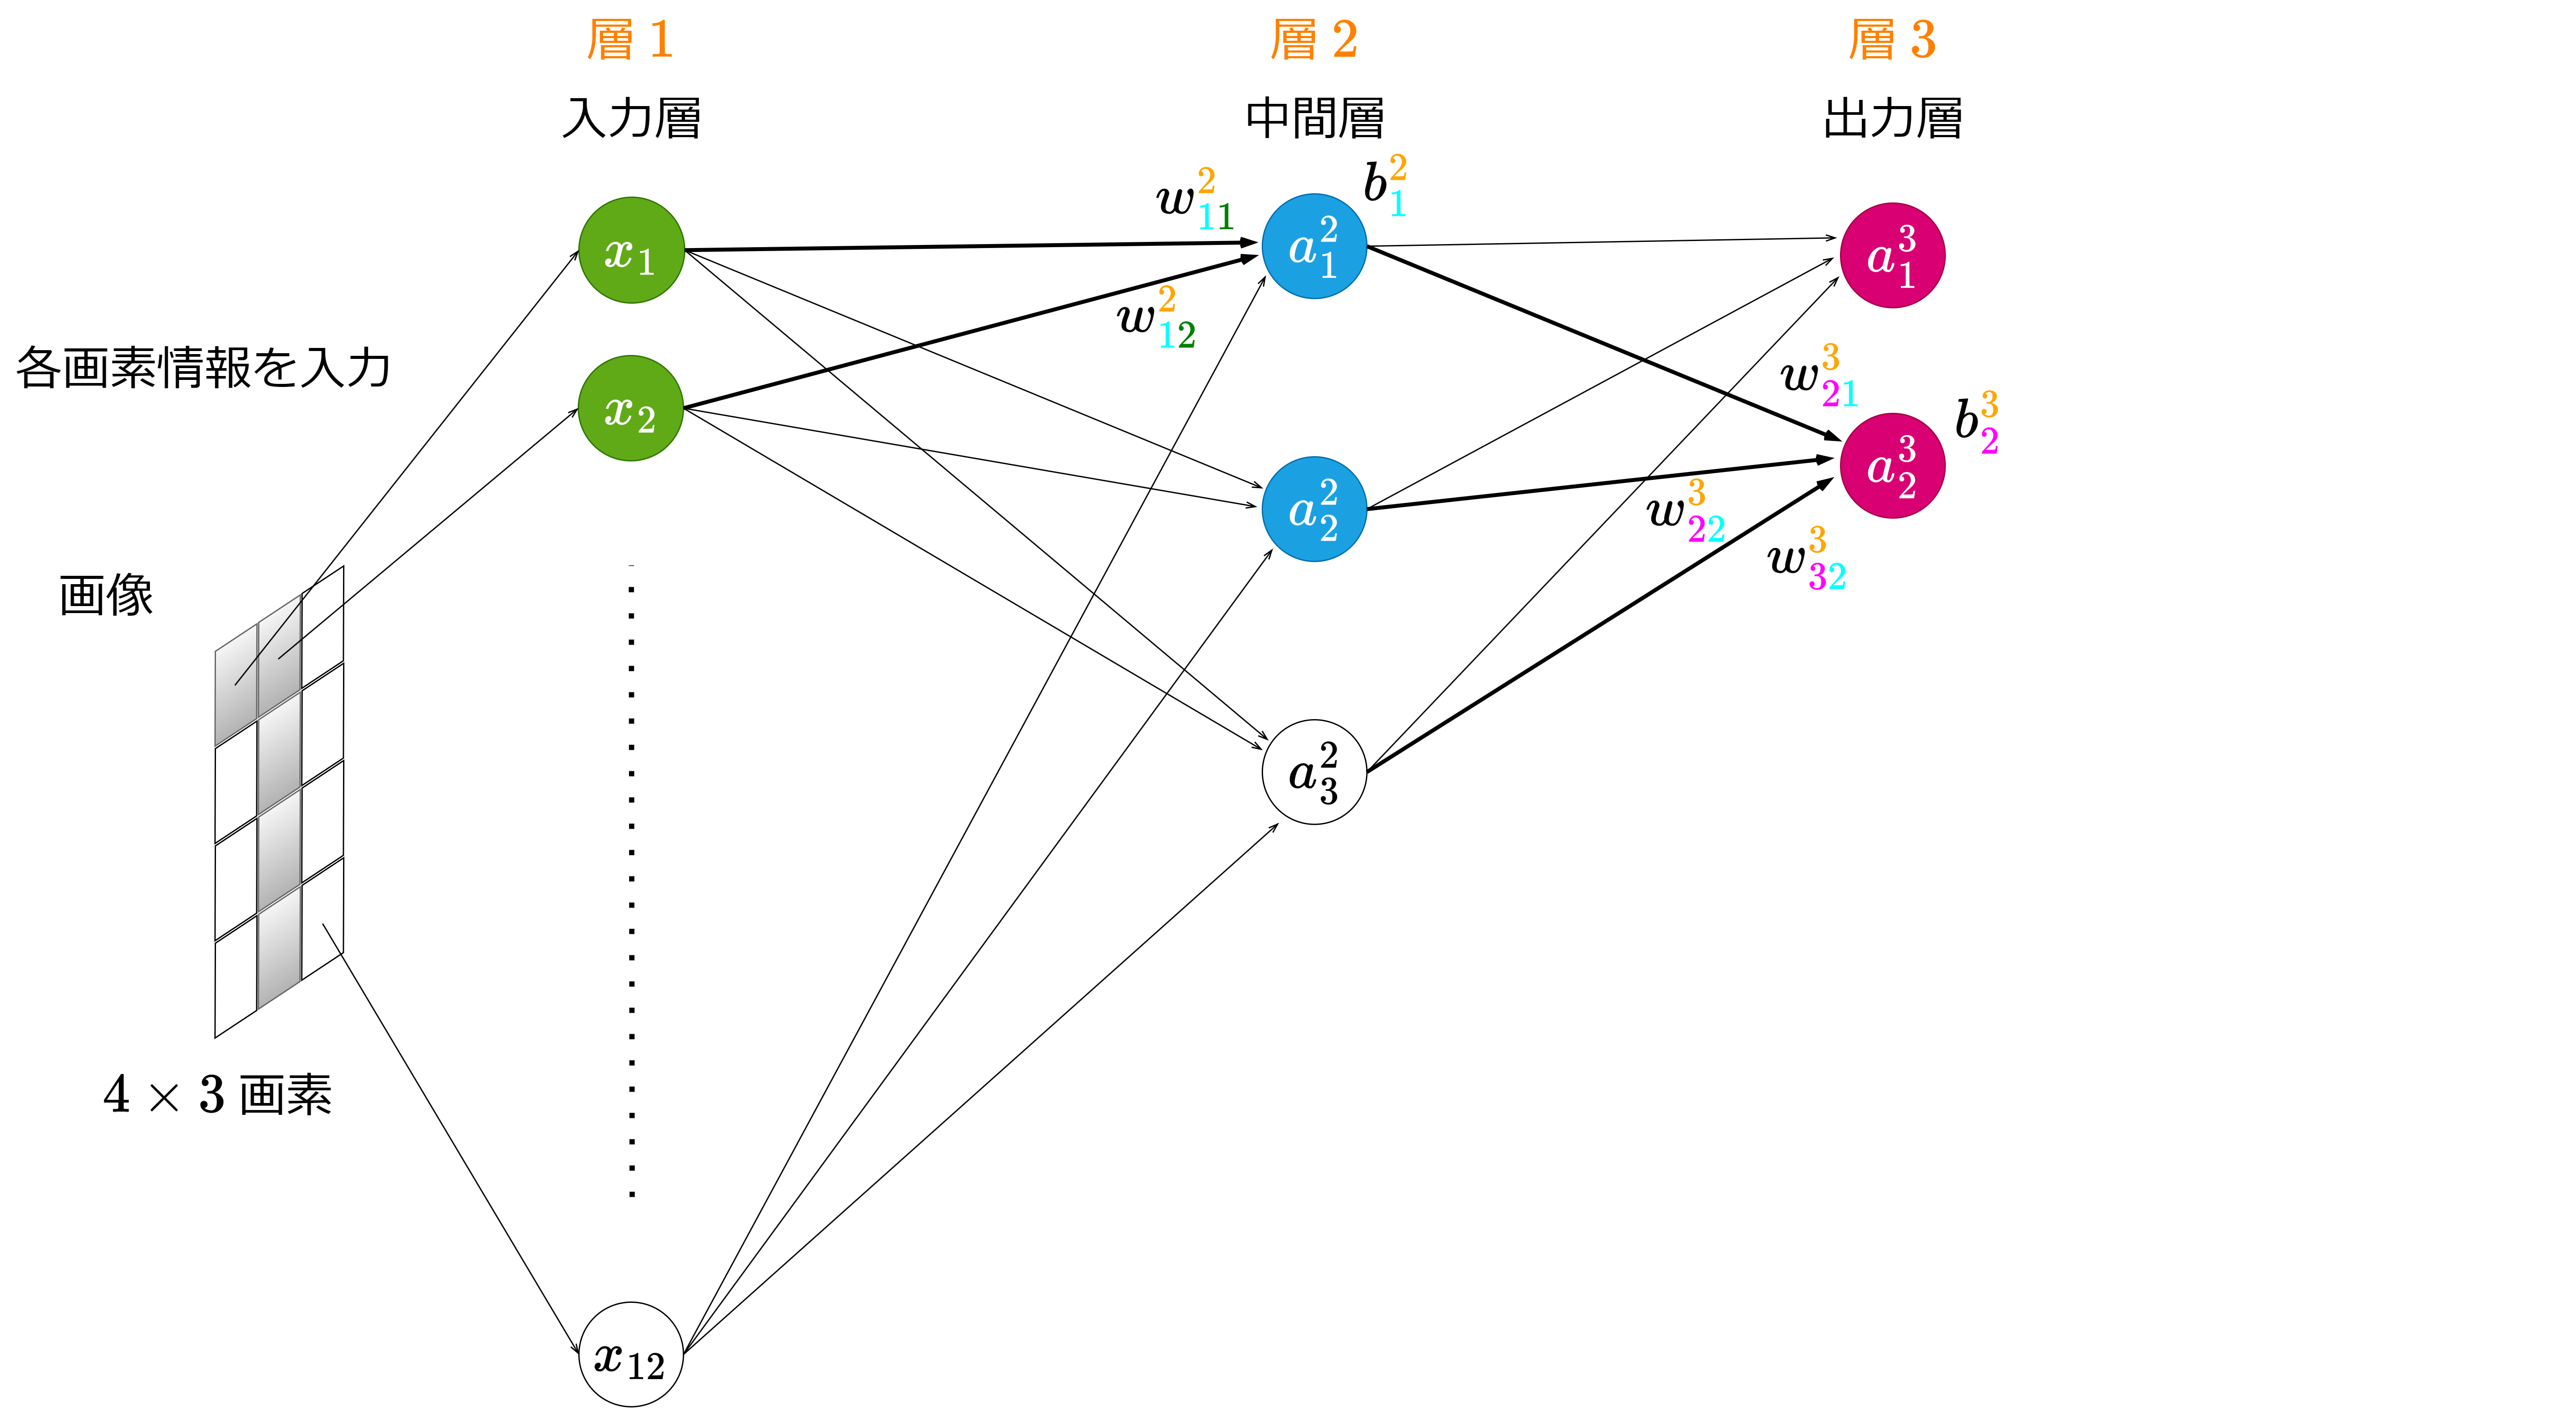
\includegraphics[width=0.8\linewidth]{img/illustration-of-variable-and-parameter-names}
		\end{figure}
	\end{frame}
	\begin{frame}{ニューラルネットワークへの勾配降下法の適用}
		$ \begin{bmatrix}
			\Delta w^2_{11}\\ \vdots\\
			\Delta w^3_{11}\\ \vdots\\
			\Delta b^2_1\\ \vdots\\
			\Delta b^3_1\\ \vdots
		\end{bmatrix} = -\eta \begin{bmatrix}
			\dfrac{\partial C_\mathrm{T}}{\partial w^2_{11}}\\ \vdots\\
			\dfrac{\partial C_\mathrm{T}}{\partial w^3_{11}}\\ \vdots\\
			\dfrac{\partial C_\mathrm{T}}{\partial b^2_1}\\ \vdots\\
			\dfrac{\partial C_\mathrm{T}}{\partial b^3_1}\\ \vdots\\
		\end{bmatrix} $を用いて、$ \begin{bmatrix}
			w^2_{11}\\ \vdots\\
			w^3_{11}\\ \vdots\\
			b^2_1\\ \vdots\\
			b^3_1\\ \vdots
		\end{bmatrix} $を$ \begin{bmatrix}
			w^2_{11} + \Delta w^2_{11}\\ \vdots\\
			w^3_{11} + \Delta w^3_{11}\\ \vdots\\
			b^2_1 + \Delta b^2_1\\ \vdots\\
			b^3_1 + \Delta b^3_1\\ \vdots
		\end{bmatrix} $へ更新を繰り返す。
		
		※正の小さな定数$ \eta $を\alert{学習係数}といい、モデル作成者が自由に設定する。
	\end{frame}
	\begin{frame}{勾配降下法の問題点}
		\underline{微分を実際に計算するのは大変}
		\begin{align*}
			\dfrac{\partial C_\mathrm{T}}{\partial w^2_{11}} 
			&= \sum_{k=1}^{64} \dfrac{\partial C_k}{\partial w^2_{11}}\\
			&= \sum_{k=1}^{64}\left\{ \dfrac{\partial C_k}{\partial a^3_1[k]}\dfrac{\partial a^3_1[k]}{\partial z^3_1[k]}\dfrac{\partial z^3_1[k]}{\partial a^2_1[k]}\dfrac{\partial a^2_1[k]}{\partial z^2_1[k]}\dfrac{\partial z^2_1[k]}{\partial w^2_{11}} + \dfrac{\partial C_k}{\partial a^3_2[k]}\dfrac{\partial a^3_2[k]}{\partial z^3_2[k]}\dfrac{\partial z^3_2[k]}{\partial a^2_1[k]}\dfrac{\partial a^2_1[k]}{\partial z^2_1[k]}\dfrac{\partial a^2_1[k]}{\partial w^2_{11}} \right\}.
		\end{align*}
	\end{frame}
	\begin{frame}{微分地獄の解決策}
		\underline{\alert{誤差逆伝播法} の導入}
		% TODO: \usepackage{graphicx} required
		\begin{figure}
			\centering
			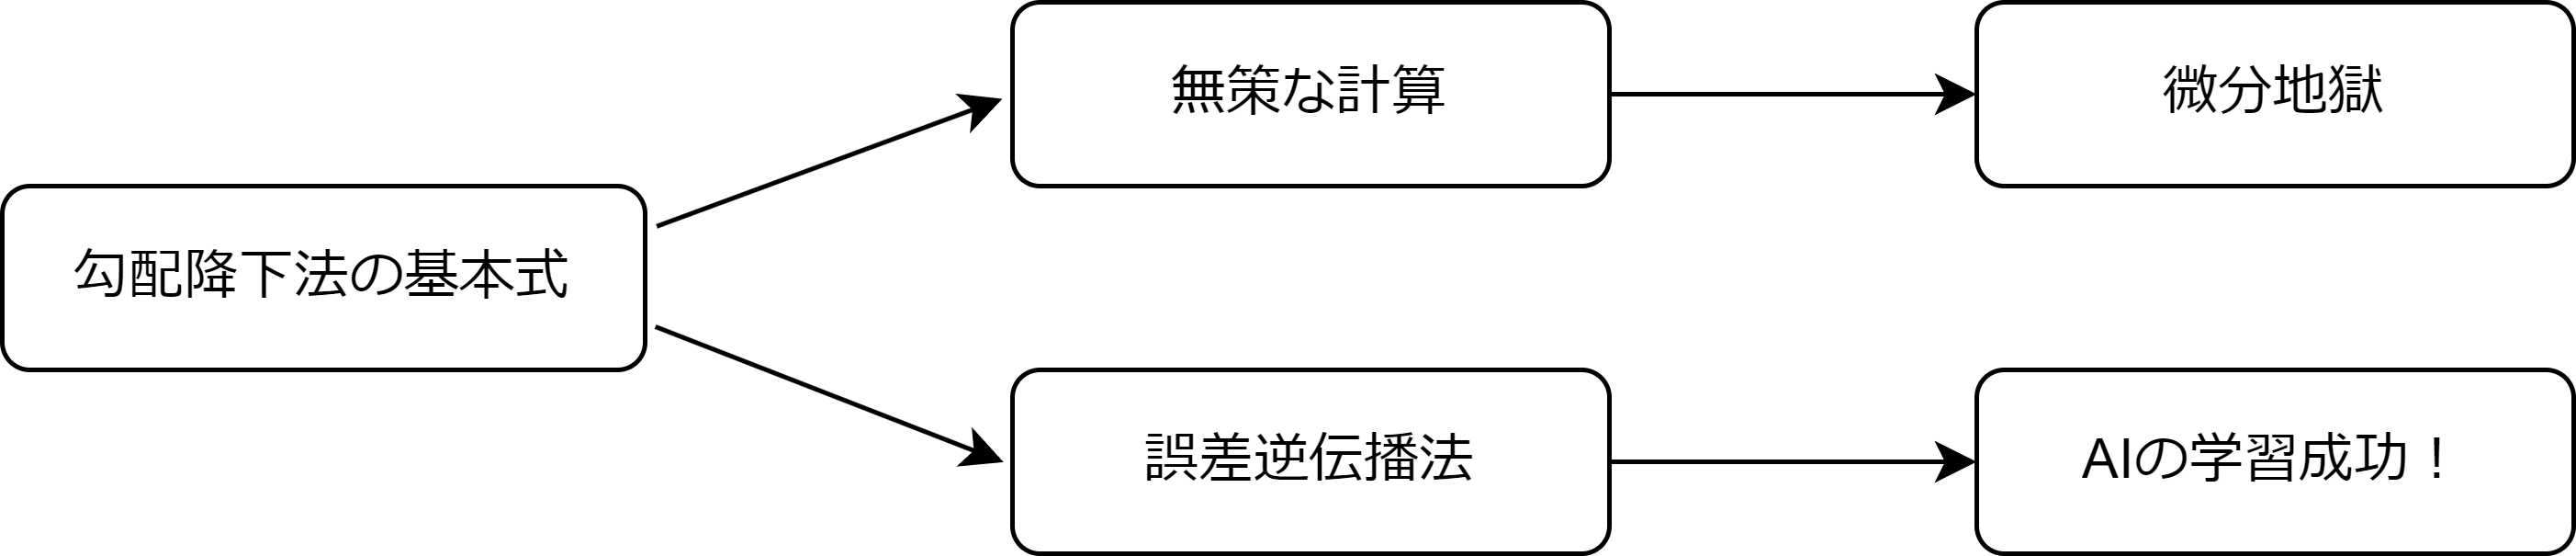
\includegraphics[width=0.9\linewidth]{img/positioning-of-the-error-back-propagation-method}
		\end{figure}
	\end{frame}
	
	\section{誤差逆伝播法}
	\subsection{ユニットの誤差}
	\begin{frame}{誤差逆伝播法とは?}
		\underline{特徴}
		\begin{itemize}
			\item 煩雑な微分計算を、\alert{数列の漸化式}に置き換える
			\item \alert{ユニットの誤差}(error)と呼ばれる変数$ \delta^l_j $を用いる
		\end{itemize}
	\end{frame}
	\begin{frame}{ユニットの誤差$ \delta^l_j $の導入}
		\begin{screen}
			\alert{ユニットの誤差}$ \delta^l_j $を次のように定義する:
			\begin{equation}\label{eq:unit-error}
				\delta^l_j \triangleq \dfrac{\partial C}{\partial z^l_j}\quad (l \geq 2).
			\end{equation}
		\end{screen}
		なぜこれを導入したか?
		\begin{itemize}
			\item 微分の計算から漸化式の計算へ変えることができるから
		\end{itemize}		
	\end{frame}
	\begin{frame}{ユニットの誤差$ \delta^l_j $のイメージ}
		% TODO: \usepackage{graphicx} required
		\begin{figure}
			\centering
			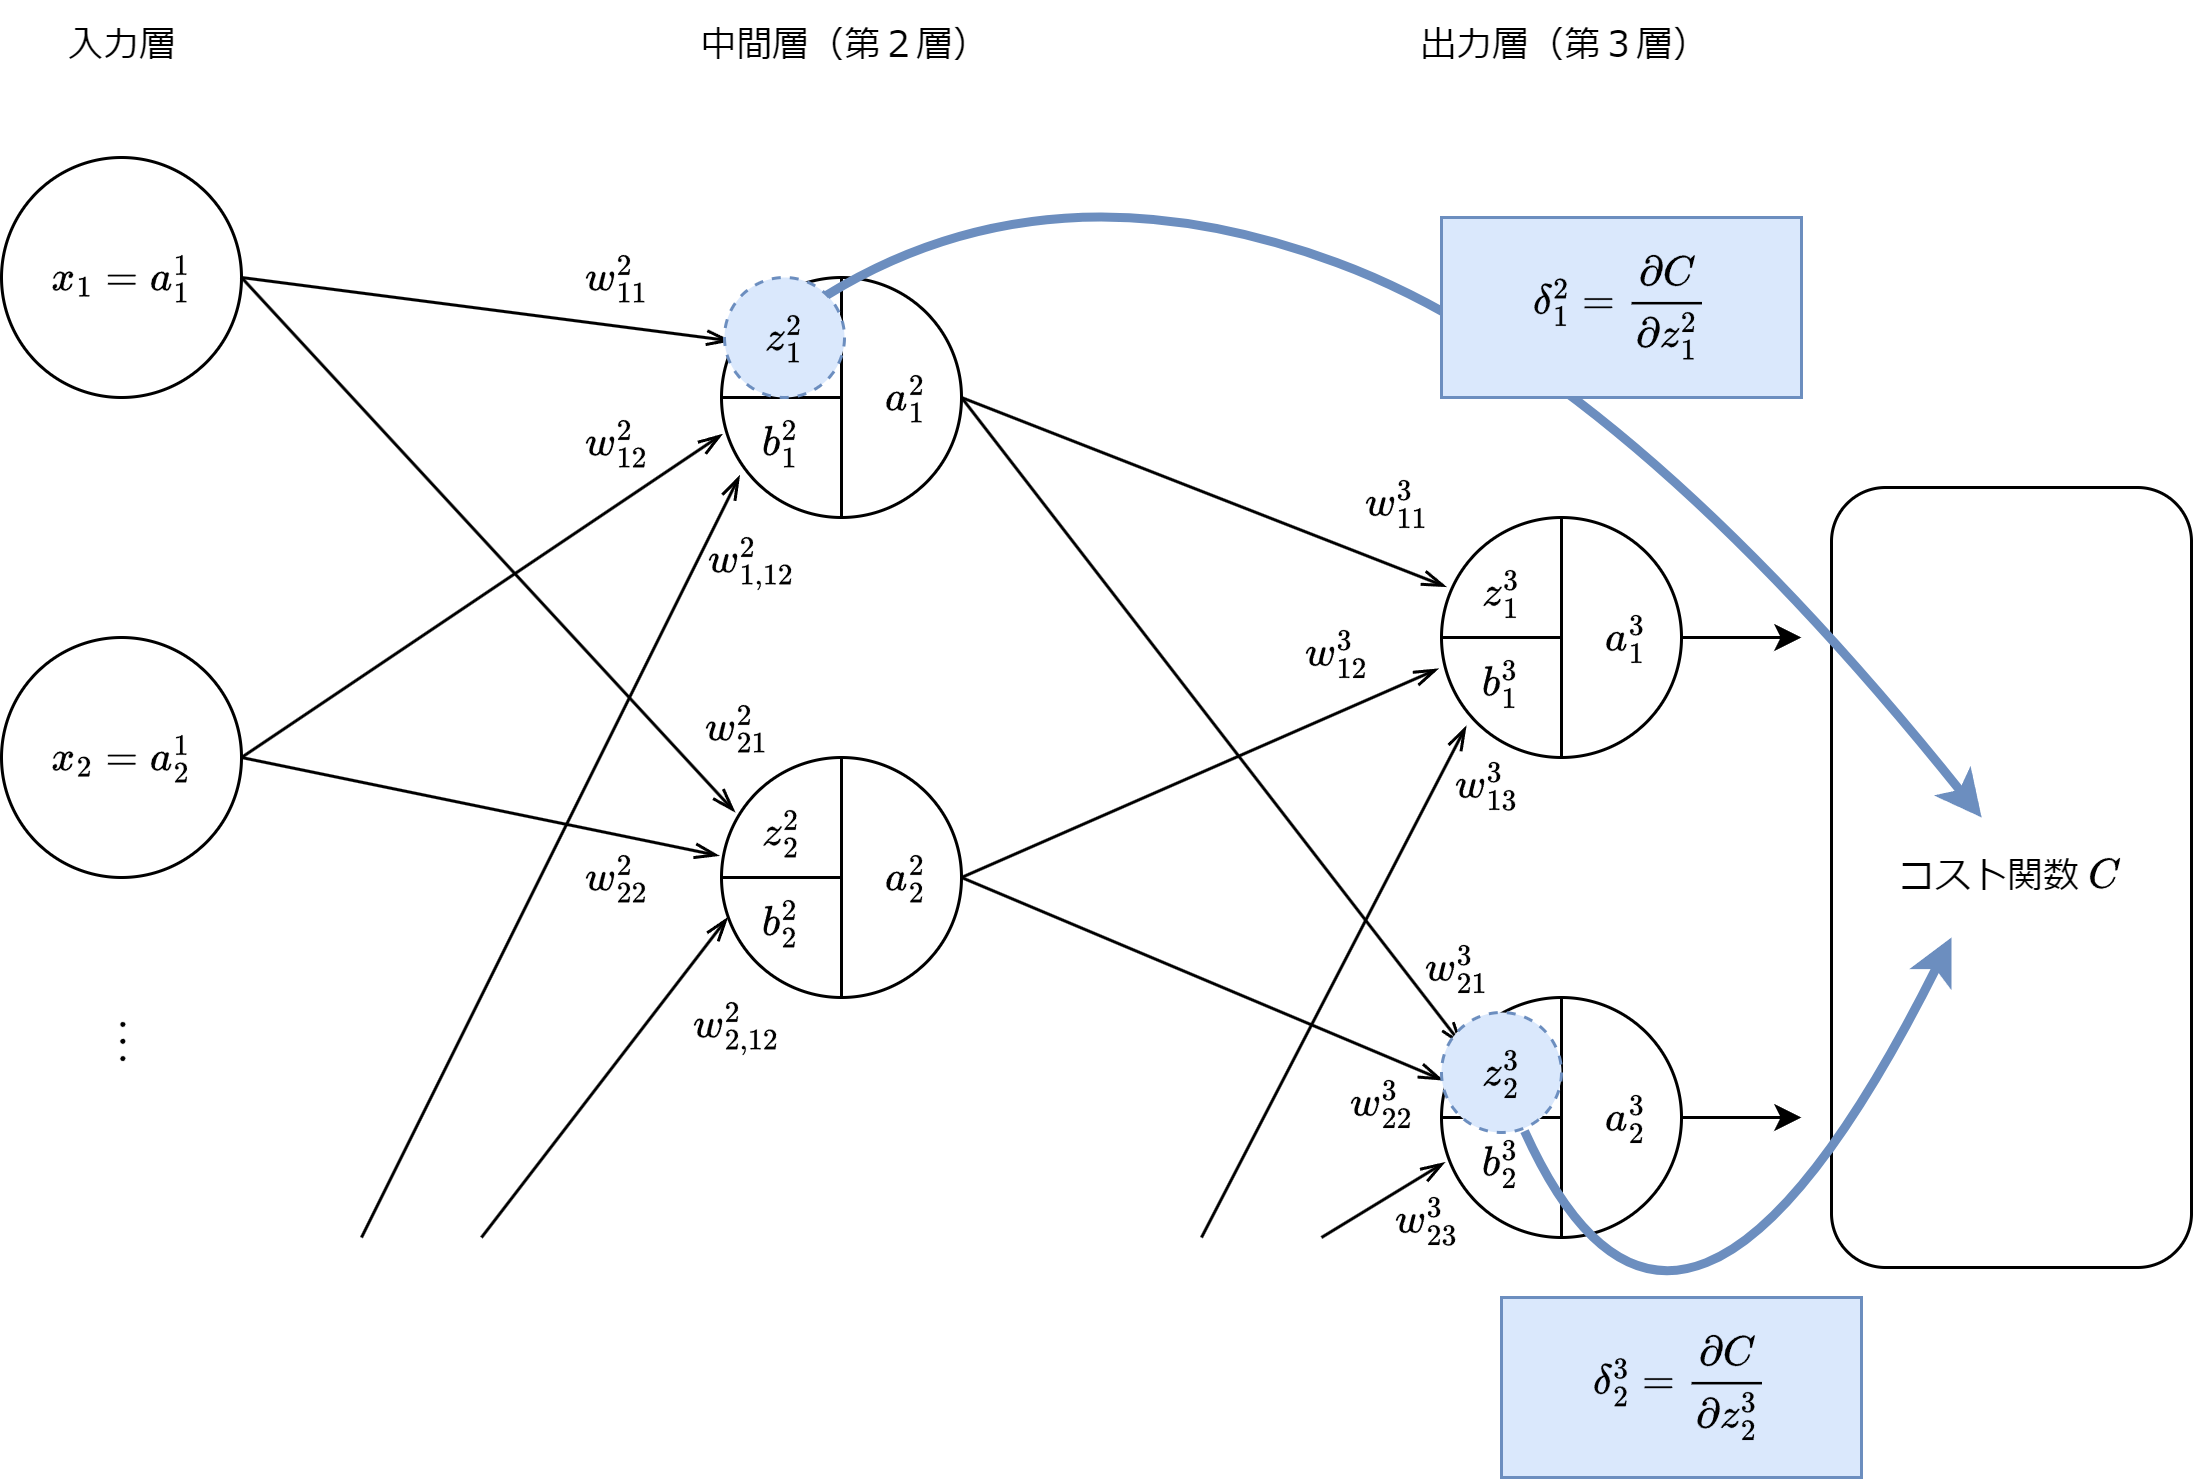
\includegraphics[width=0.7\linewidth]{img/image-of-unit-error}
		\end{figure}
	\end{frame}
	\begin{frame}{重みに関する2乗誤差の偏微分を$ \delta^l_j $で表現}
		\begin{screen}
			重みに関する偏微分をユニットの誤差$ \delta^l_j $を用いて次にように表すことができる:
			\begin{equation}\label{eq:equation-expressing-the-partial-derivative-with-respect-to-the-weights-using-the-unit-error}
				\dfrac{\partial C}{\partial w^l_{ji}} = \delta^l_j a^{l-1}_i\quad (l \geq 2).
			\end{equation}
		\end{screen}
		\underline{ポイント}
		\begin{itemize}
			\item $ \delta^l_j $の値さえ計算できれば、$ \dfrac{\partial C}{\partial w^l_{ji}} $を偏微分の計算なしで求めることができる!
			\begin{itemize}
				\item $ a^{l-1}_i $はユニットの出力値なので、普通に計算できる
			\end{itemize}
		\end{itemize}
	\end{frame}
	\begin{frame}{重みに関する2乗誤差の偏微分のイメージ}
		% TODO: \usepackage{graphicx} required
		\begin{figure}
			\centering
			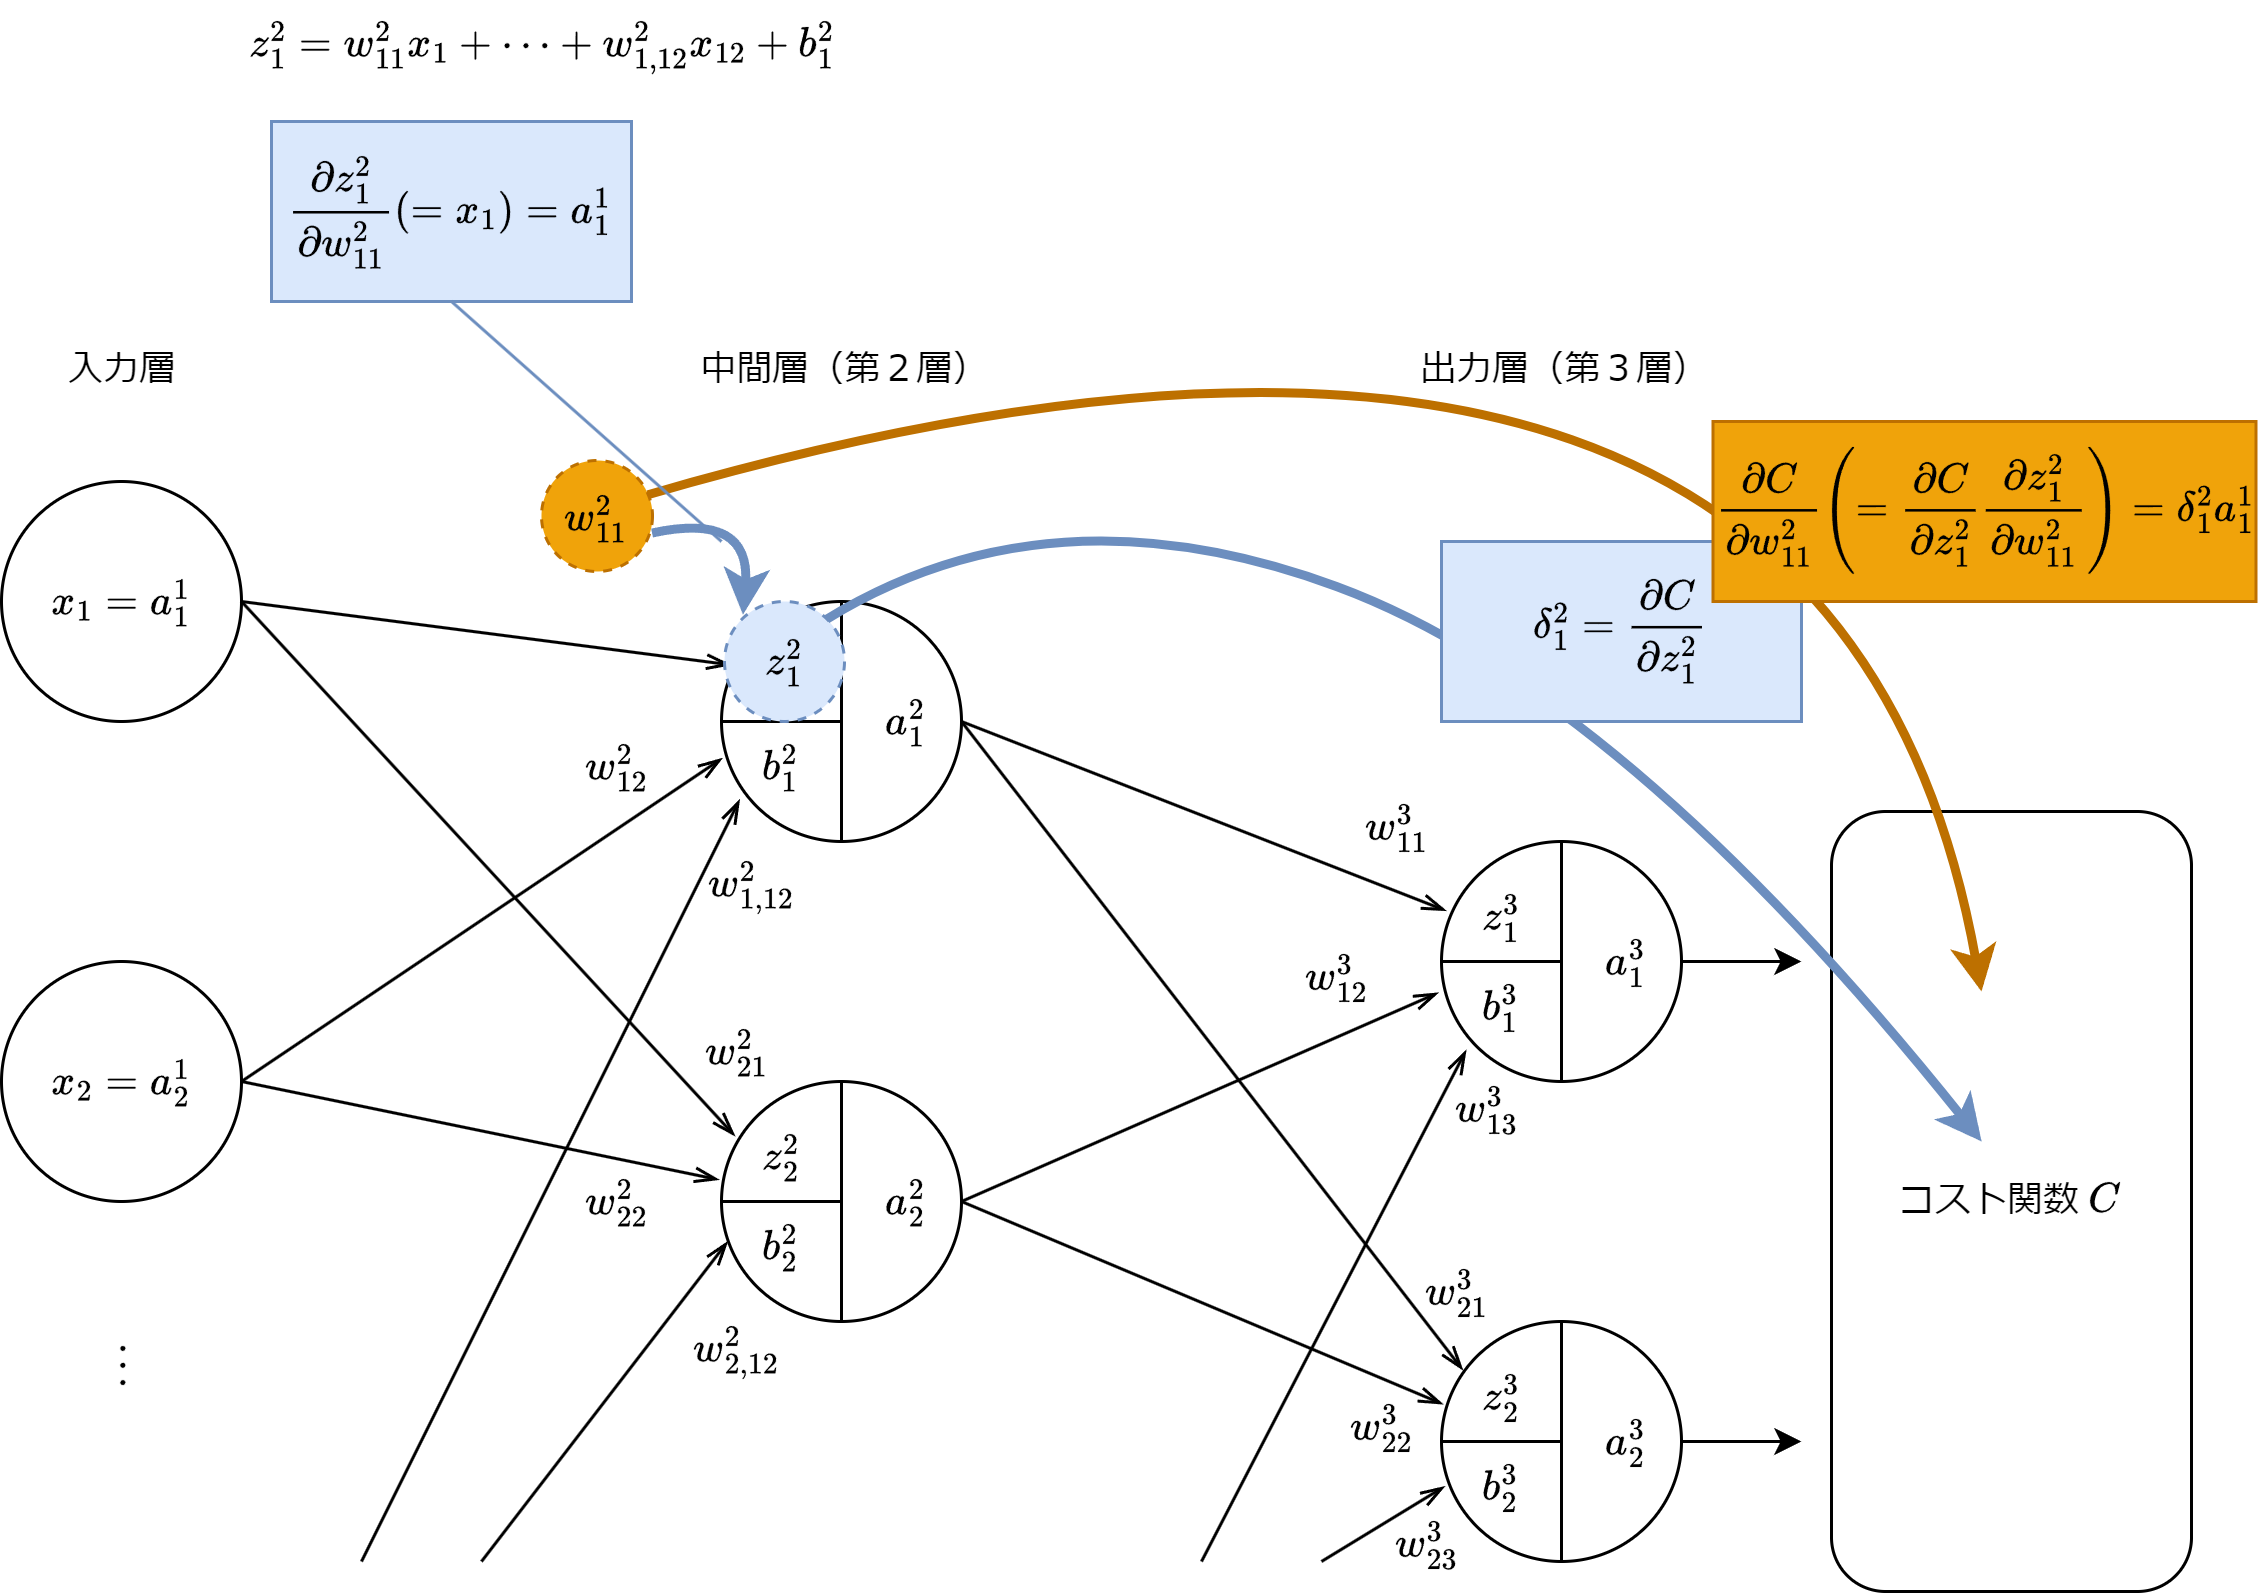
\includegraphics[width=0.7\linewidth]{img/image-of-the-partial-derivative-of-the-squared-error-with-respect-to-the-weights}
		\end{figure}
	\end{frame}
	\begin{frame}{バイアスに関する2乗誤差の偏微分を$ \delta^l_j $で表現}
		\begin{screen}
			バイアスに関する偏微分をユニットの誤差$ \delta^l_j $を用いて次にように表すことができる:
			\begin{equation}\label{eq:equation-expressing-the-partial-derivative-with-respect-to-the-bias-using-the-unit-error}
				\dfrac{\partial C}{\partial b^l_j} = \delta^l_j\quad (l \geq 2).
			\end{equation}
		\end{screen}
		ポイント
		\begin{itemize}
			\item $ \delta^l_j $の値さえ計算できれば、$ \dfrac{\partial C}{\partial b^l_j} $を偏微分の計算なしで求めることができる!
		\end{itemize}
	\end{frame}
	\begin{frame}{バイアスに関する2乗誤差の偏微分のイメージ}
		% TODO: \usepackage{graphicx} required
		\begin{figure}
			\centering
			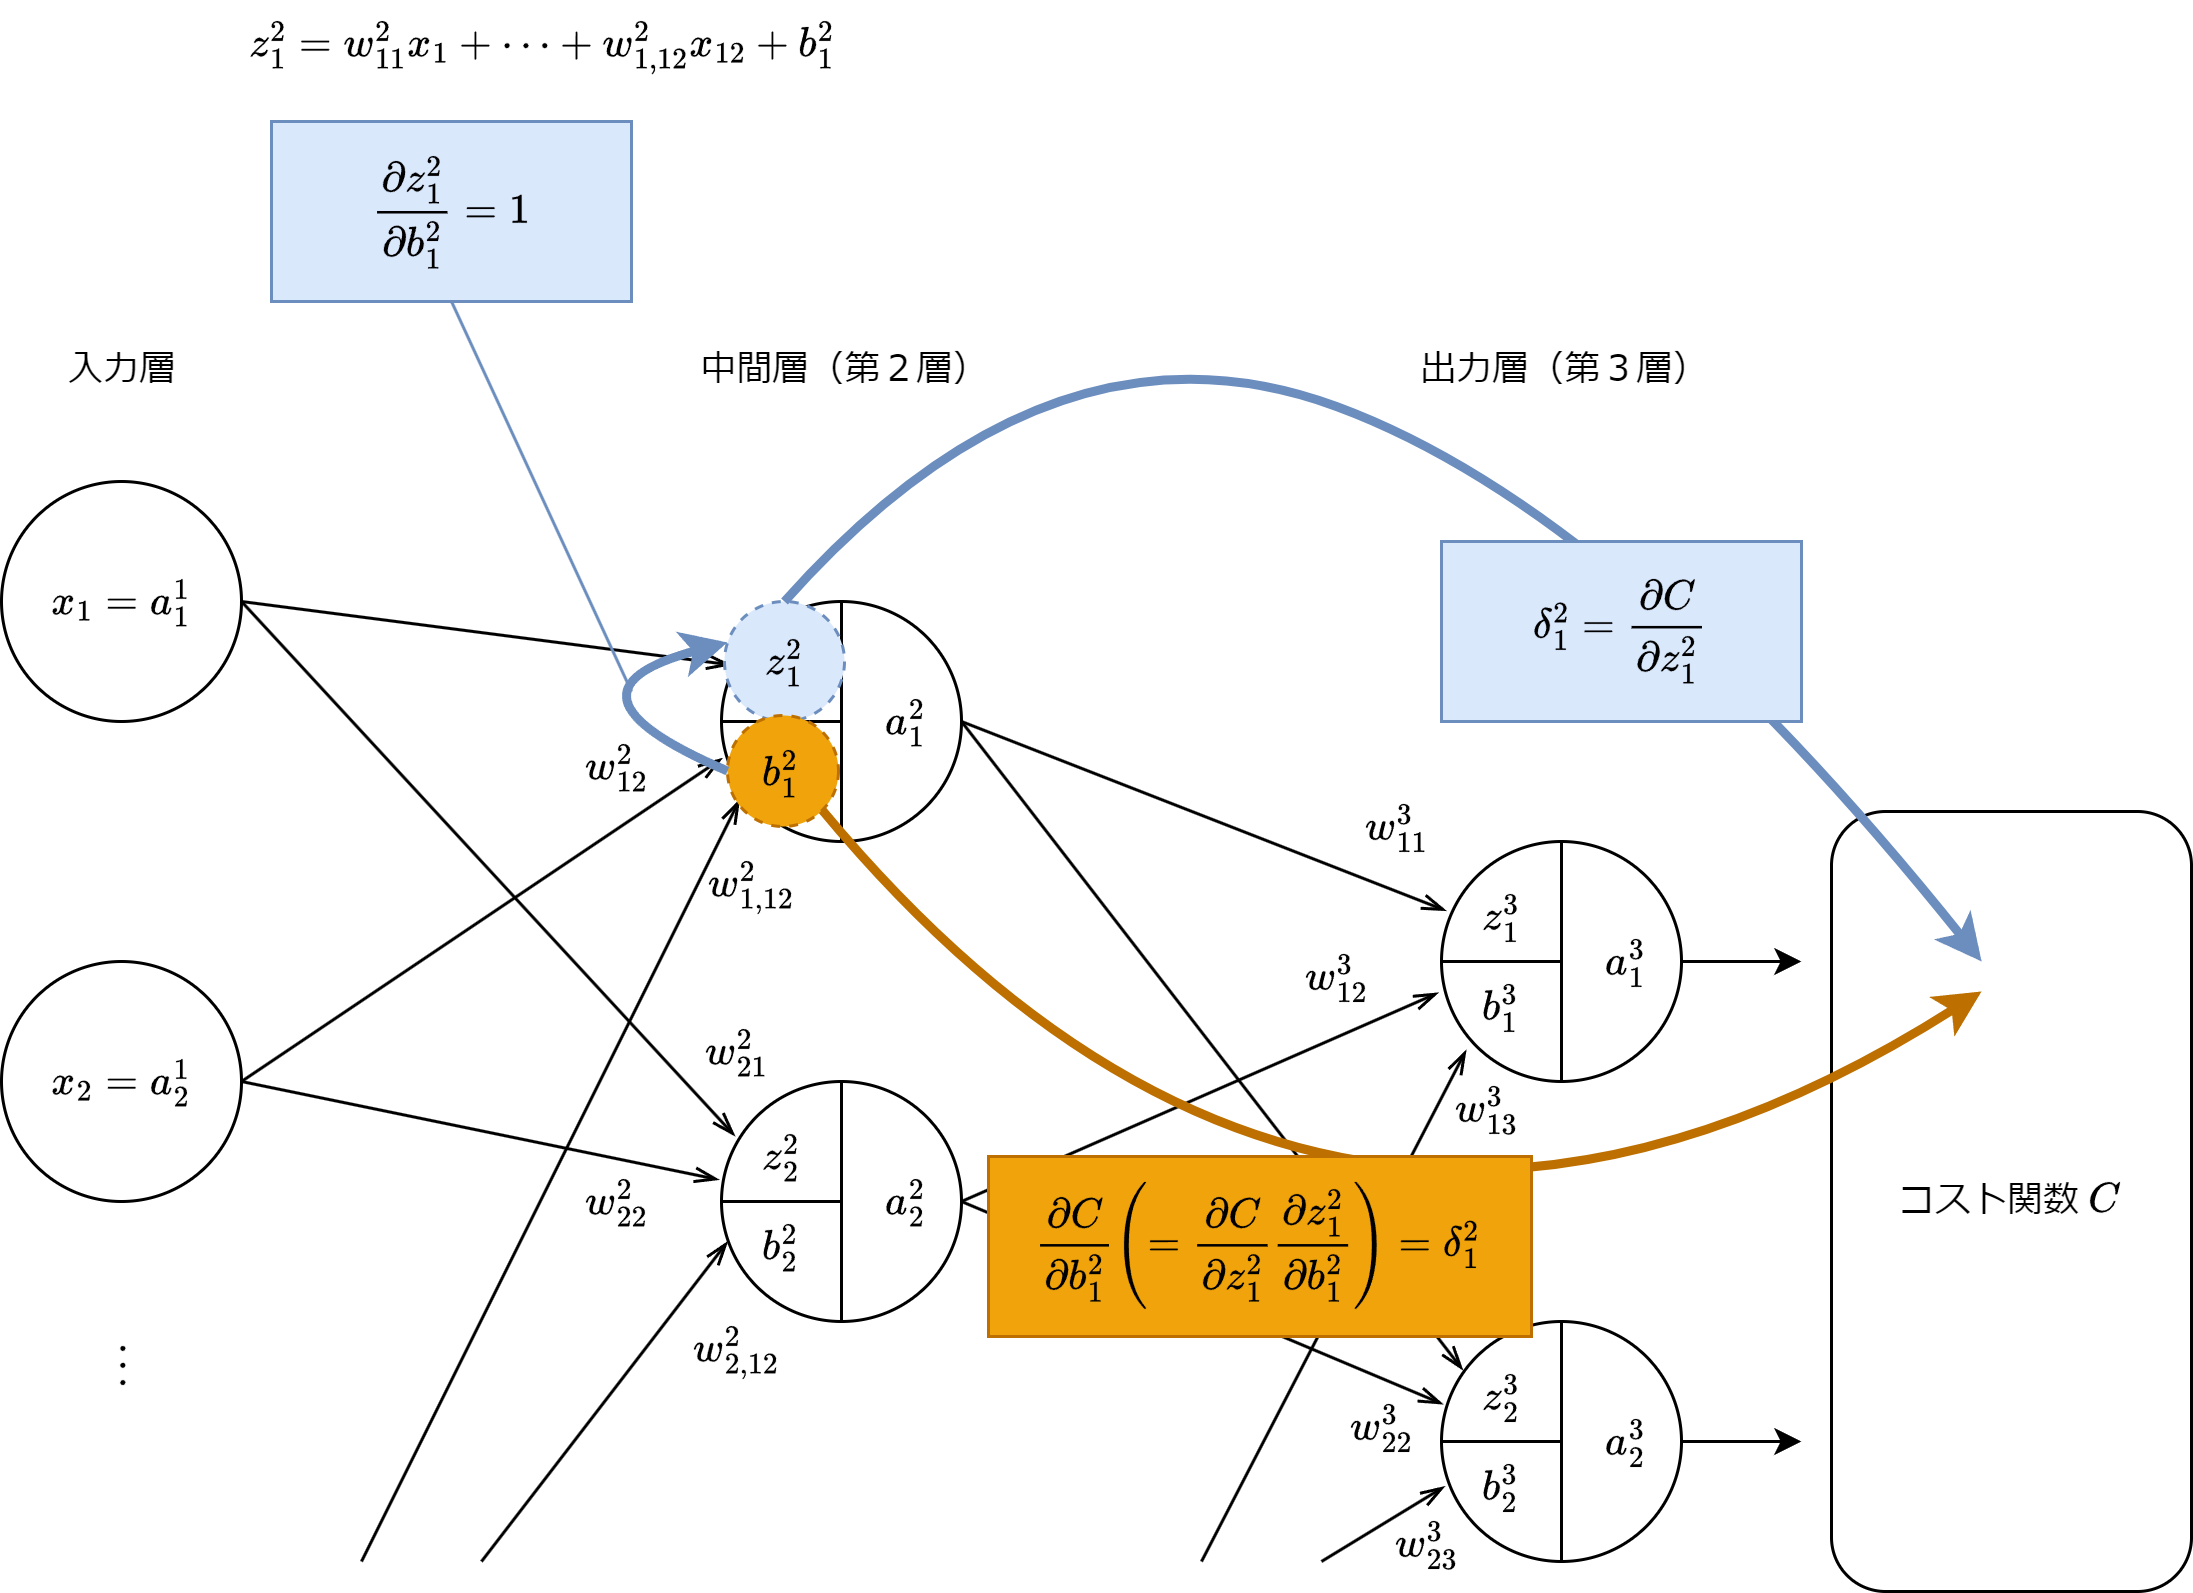
\includegraphics[width=0.7\linewidth]{img/image-of-the-partial-derivative-of-the-squared-error-with-respect-to-the-bias}
		\end{figure}
	\end{frame}
	\begin{frame}{で、$ \delta^l_j $はどう計算するの?}
		\underline{ここでようやく\alert{漸化式}の考え方が役立つ!}
		\begin{enumerate}
			\item 出力層(第$ L $層)のユニットの誤差$ \delta^L_j $を計算する
			\item $ l $層と$ l+1 $層のユニットの誤差の「(逆)漸化式」を用いて、出力層側のユニットの誤差から入力層側のユニットの誤差を計算する
		\end{enumerate}
		つまり、$ \delta^L_j $が計算できれば、$ \delta^{L-1}_j, \delta^{L-2}_j,\dots, \delta^2_j $とすべて計算できることになる
	\end{frame}
	\begin{frame}{【重要】出力層の$ \delta^L_j $}
		\begin{screen}
			出力層のユニットの誤差$ \delta^L_j $は次にように表すことができる:
			\begin{align}\label{eq:output-layer-unit-error}
				\delta^L_j 	&= \dfrac{\partial C}{\partial a^L_j} \dfrac{\mathrm{d} a^L_j}{\mathrm{d}z^L_j}\notag\\
							&= (a^L_j - t_j)\cdot\sigma(z^L_j)\cdot\left\lbrace1 - \sigma(z^L_j)\right\rbrace.
			\end{align}
		\end{screen}
		\underline{ポイント}
		\begin{itemize}
			\item $ a^L_j,\ t_j,\ z^L_j $はすべて分かっている!数値計算可能!!
		\end{itemize}
	\end{frame}
	\begin{frame}{出力層の$ \delta^L_j $のイメージ}
		% TODO: \usepackage{graphicx} required
		\begin{figure}
			\centering
			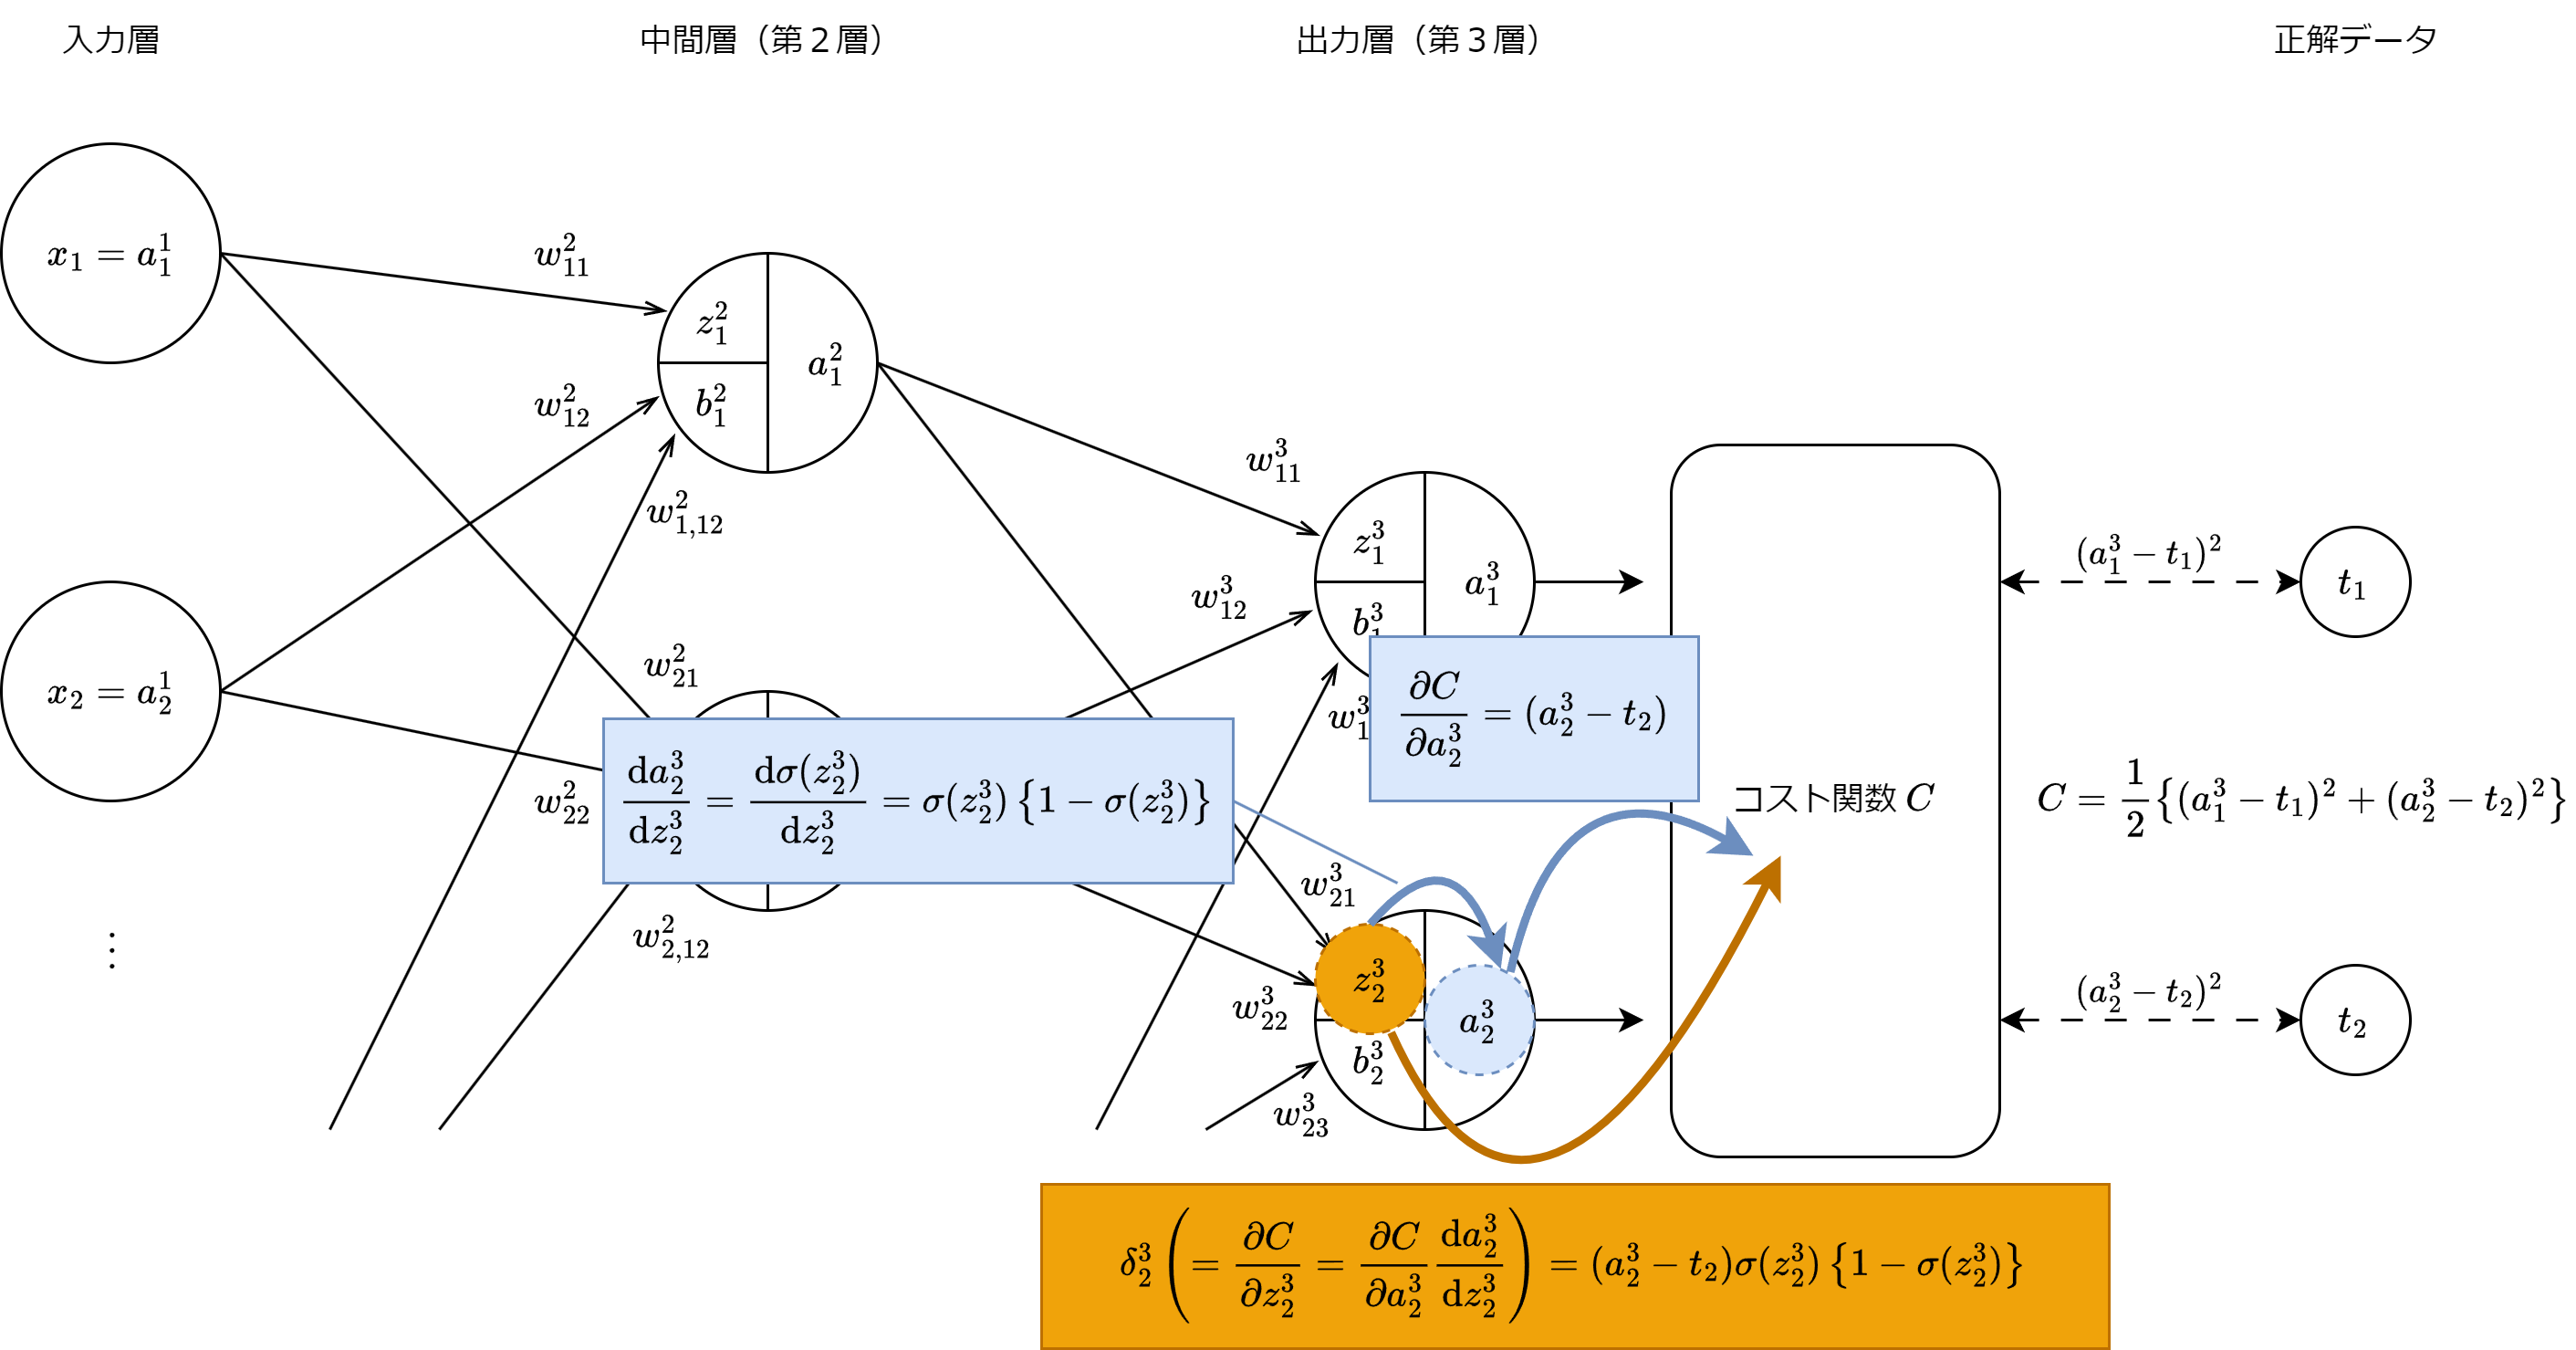
\includegraphics[width=1.0\linewidth]{img/image-of-output-layer-unit-error}
		\end{figure}
	\end{frame}
	\begin{frame}{中間層の$ \delta^l_j $}
		\begin{screen}
			中間層のユニットの誤差$ \delta^l_i $は次のように表すことができる:
			\begin{align}
				\delta^l_i 	&= \dfrac{\mathrm{d}a^l_i}{\mathrm{d}z^l_i} \sum_j \delta^{l+1}_j w^{l+1}_{ji}\notag\\
				 			&= \sigma(z^l_i) \cdot \left\lbrace 1 - \sigma(z^l_i) \right\rbrace \cdot \sum_j \delta^{l+1}_j w^{l+1}_{ji}\quad (l \geq 2).\label{eq:hidden-layer-unit-error}
			\end{align}
		\end{screen}
	\end{frame}
	\begin{frame}{中間層の$ \delta^l_i $のイメージ}
		% TODO: \usepackage{graphicx} required
		\begin{figure}
			\centering
			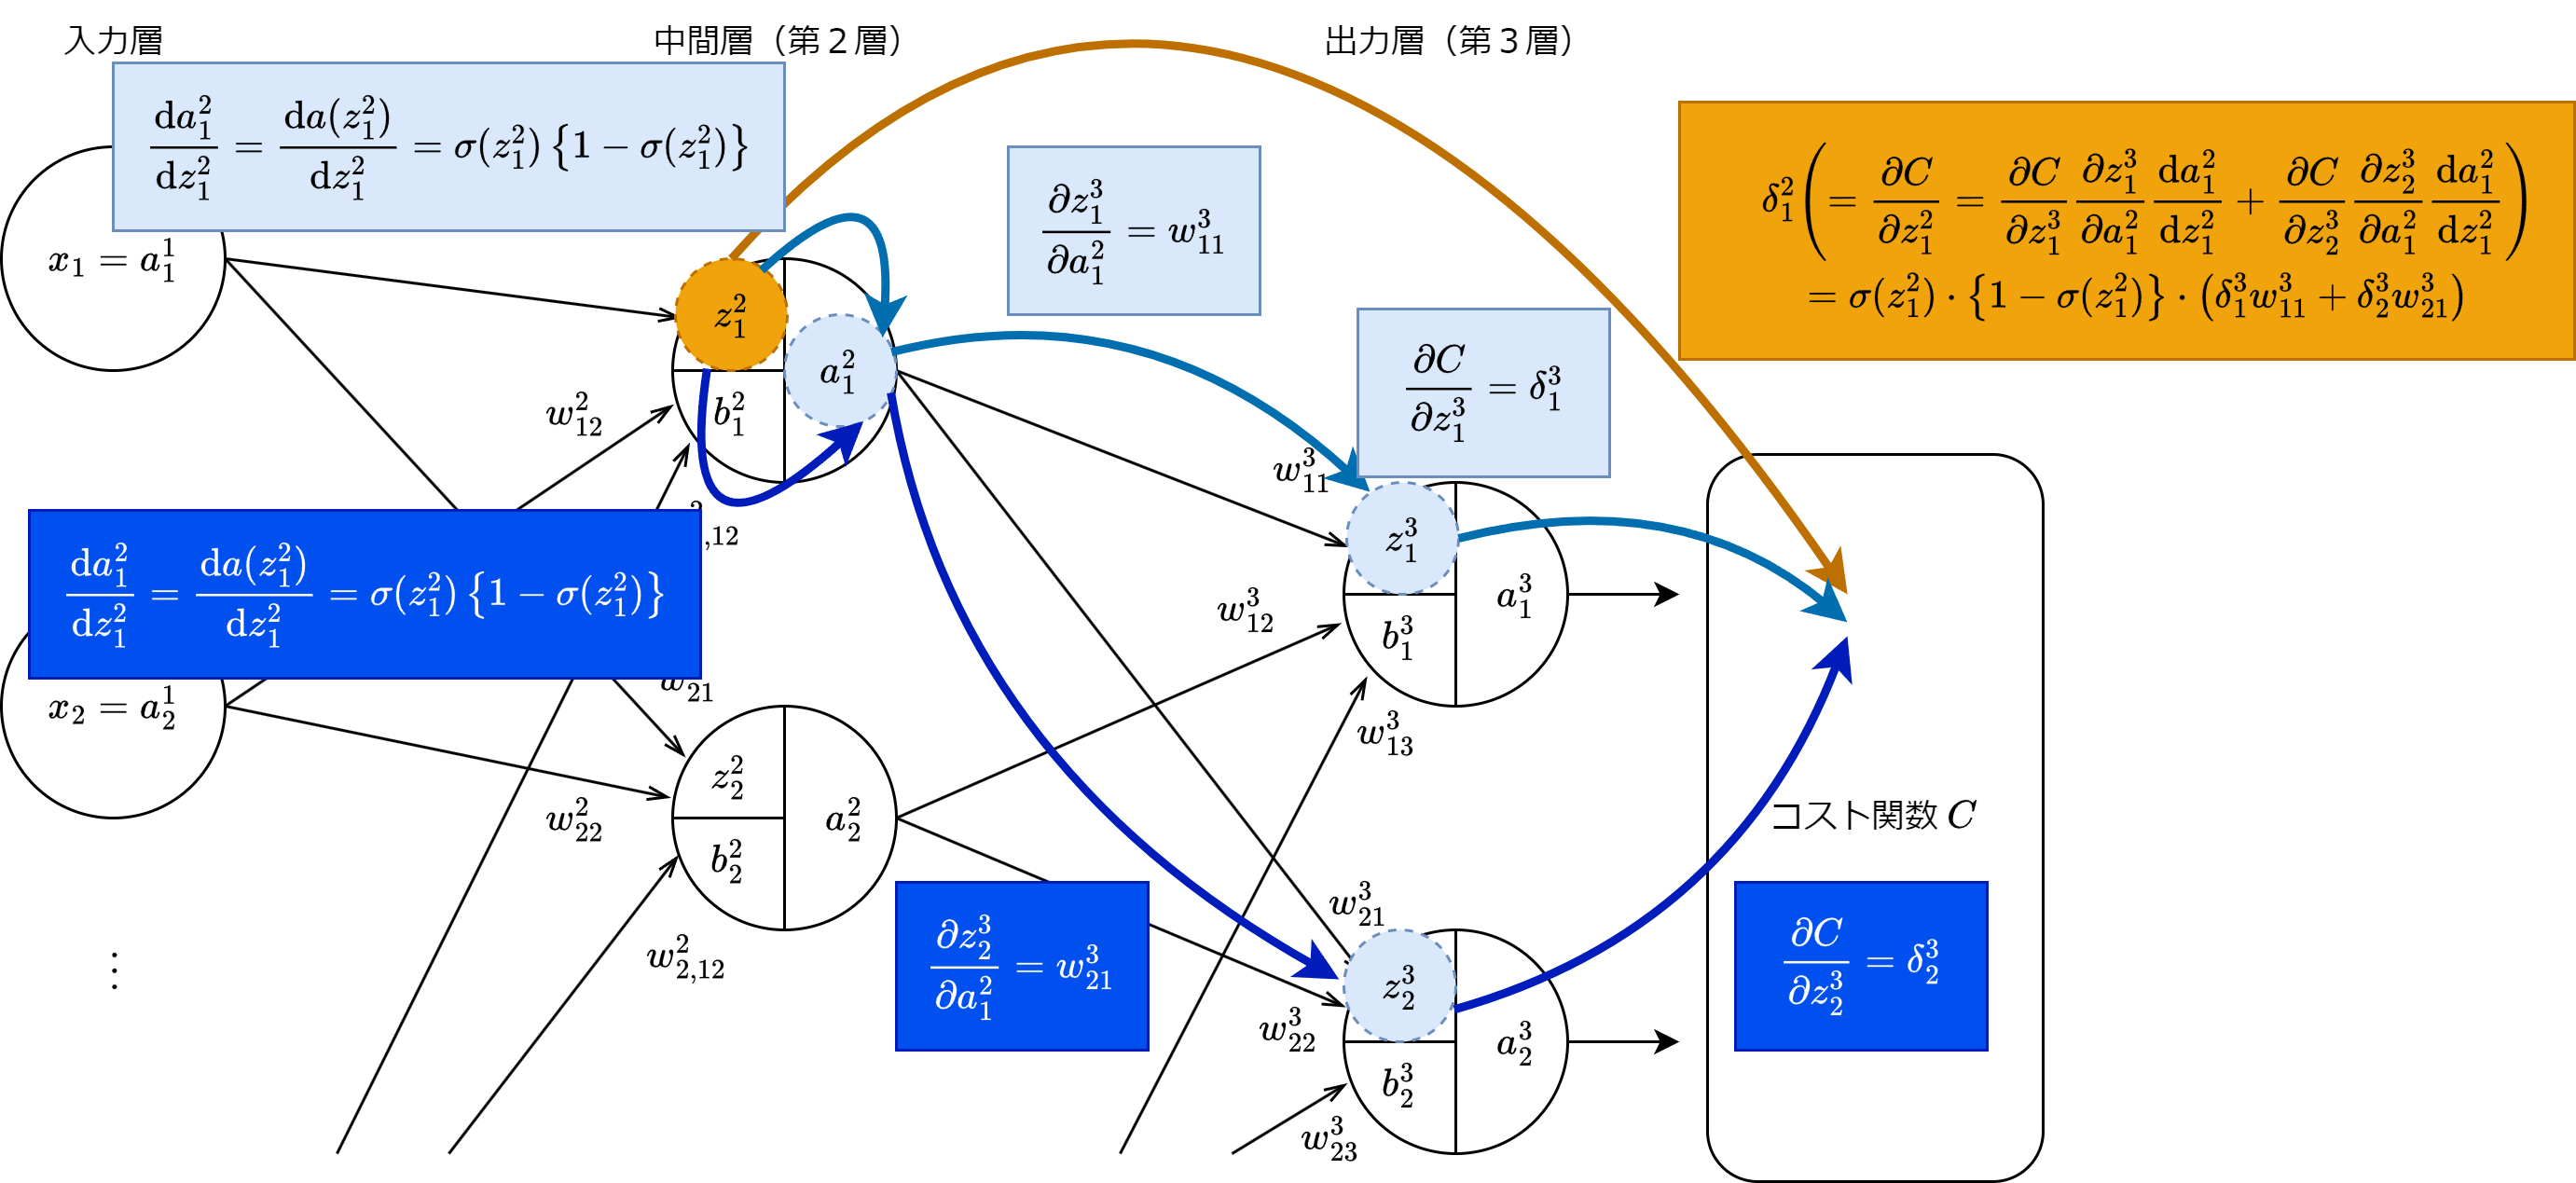
\includegraphics[width=\linewidth]{img/Image-of-hidden-layer-unit-error}
		\end{figure}
	\end{frame}
	\begin{frame}{中間層の$ \delta^l_i $の式をどう使う?}
		式\eqref{eq:hidden-layer-unit-error}で$ l+1 = L $とすると、
		\begin{equation*}
			\delta^{L-1}_i = \sigma(z^{L-1}_i)\left\lbrace 1 - \sigma(z^{L-1}_i) \right\rbrace \sum_j \delta^L_j w^L_{ji}.
		\end{equation*}
		\begin{itemize}
			\item $ z^{L-1}_i $はニューラルネットワークの重み付き入力なので、計算済み
			\item $ w^L_{ji} $はニューラルネットワークの重みなので、ただの数字
			\item $ \delta^L_j $は出力層のユニットの誤差なので、計算可能(式\eqref{eq:output-layer-unit-error})
		\end{itemize}
		$ \delta^L_j $が求まれば$ \delta^{L-1}_i, \delta^{L-2}_i, \dots, \delta^2_i $とすべてのユニットの誤差$ \delta^l_i $を求めることができる!
	\end{frame}
	\begin{frame}{$ \delta^l_i $が計算できるようになると、、、?}
		\begin{itemize}
			\item 
				式\eqref{eq:equation-expressing-the-partial-derivative-with-respect-to-the-weights-using-the-unit-error}, \eqref{eq:equation-expressing-the-partial-derivative-with-respect-to-the-bias-using-the-unit-error}を用いて$ \dfrac{\partial C}{\partial w^l_{ji}} $も$ \dfrac{\partial C}{\partial b^l_j} $も\underline{微分なしで}計算できる!
			\item
				勾配降下法の微分地獄を回避できた!!
		\end{itemize}
	\end{frame}
	\subsection{アルゴリズム}
	\begin{frame}[shrink]{誤差逆伝播法のアルゴリズム}
		\begin{enumerate}
			\item 学習データ・正解データの用意
			\item 重み$ (w^l_{ji}) $・バイアス$ (b^l_j) $をランダムに、学習率$ \eta $を小さい正の値で設定
			\item 重み付き入力$ (z^l_j[k]) $、活性化関数の値$ (a^l_j[k]) $、2乗誤差$ (C_k) $を算出
			\item 式\eqref{eq:output-layer-unit-error}を用いて出力層の「ユニットの誤差」$ (\delta^L_j[k]) $、式\eqref{eq:hidden-layer-unit-error}を用いて中間層の「ユニットの誤差」$ (\delta^l_i[k]) $を算出
			\item 式\eqref{eq:equation-expressing-the-partial-derivative-with-respect-to-the-weights-using-the-unit-error},\ \eqref{eq:equation-expressing-the-partial-derivative-with-respect-to-the-bias-using-the-unit-error}を用いて、ユニットの誤差から2乗誤差$ \{C_k\} $の偏微分$ \left( \dfrac{\partial C_k}{\partial w^l_{ji}} \right),\ \left( \dfrac{\partial C_k}{\partial b^l_j} \right) $を算出
			\item 3.~5. のデータを足し合わせることでコスト関数$ C_\mathrm{T} $を算出し、その勾配成分$ (\Delta w^l_{ji}) = -\eta\left( \dfrac{\partial C_\mathrm{T}}{\partial w^l_{ji}} \right),\ (\Delta b^l_j) = -\eta\left( \dfrac{\partial C_\mathrm{T}}{\partial b^l_j} \right) $を算出\footnote{この勾配成分をまとめたベクトル(勾配)を$ \nabla C_\mathrm{T} $と表す。}
			\item 勾配降下法を利用して、6. で求めた勾配成分から重みとバイアスの値を更新
			\item コスト関数$ C_\mathrm{T} $が十分小さくなるまで、3.~7. を反復\vspace{1em}
		\end{enumerate}
	\end{frame}
	\begin{frame}{1. 学習データ・正解データを用意}
		% TODO: \usepackage{graphicx} required
		\begin{figure}
			\centering
			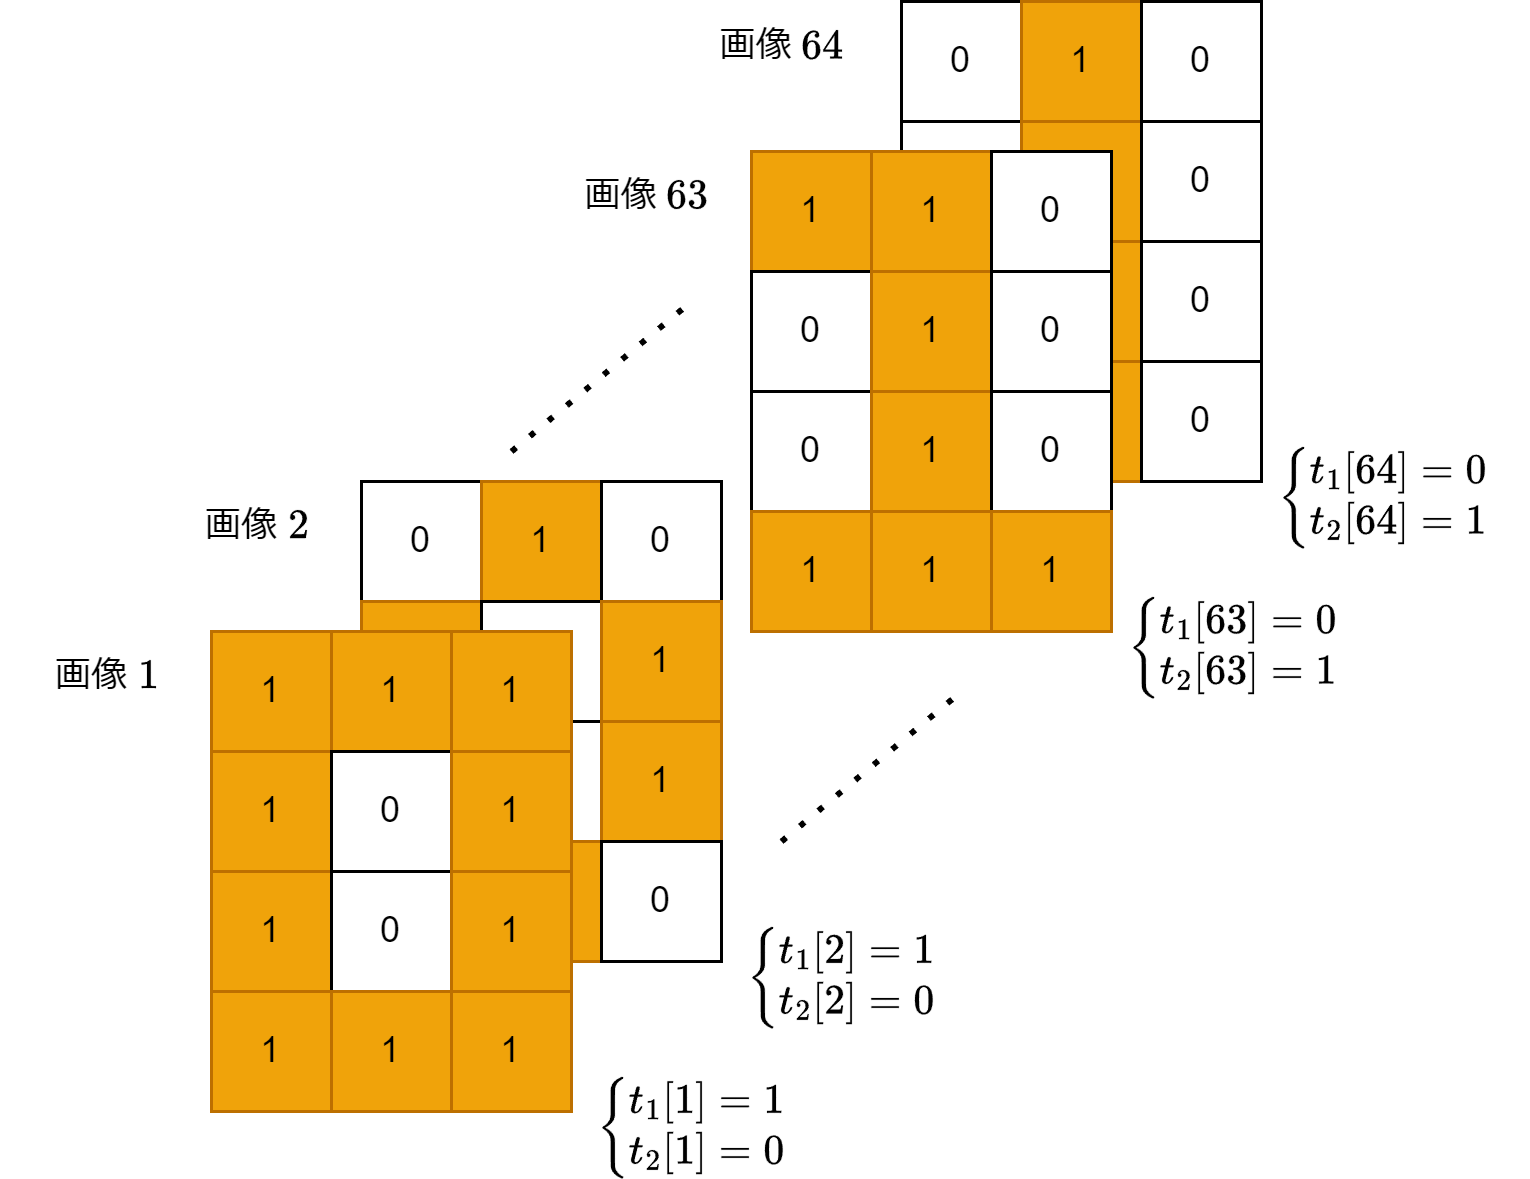
\includegraphics[width=0.65\linewidth]{img/prepare-training-data}
		\end{figure}
	\end{frame}
	\begin{frame}{2. 重み、バイアス、学習率の初期設定}
		\begin{itemize}
			\item $ w^l_{ji} \longleftarrow \mathrm{random} $
			\item $ b^l_j \longleftarrow \mathrm{random} $
			\item $ \eta \longleftarrow \mathrm{random} $
		\end{itemize}
	\end{frame}
	\begin{frame}{3. ユニットの出力値、活性化関数の値、2乗誤差の算出}
		\begin{itemize}
			\item $ z^l_j[k] \longleftarrow \displaystyle\sum_m w^l_{jm}a^{l-1}_m[k] + b^l_j,\quad a^1_j[k] = x_j[k] $
			\item $ a^l_j[k] \longleftarrow \sigma(z^l_j[k]) = \dfrac{1}{1 + e^{-z^l_j[k]}} $
			\item $ C_k \longleftarrow \dfrac{1}{2} \displaystyle\sum_m \left( t_m[k] - a^L_m[k] \right)^2 $
		\end{itemize}
	\end{frame}
	\begin{frame}{4. 誤差逆伝播法から各層のユニットの誤差の算出}
		\begin{itemize}
			\item $ \delta^L_j[k] \longleftarrow (t_j[k] - a^L_j[k]) \cdot \sigma(z^L_j[k]) \cdot\left\lbrace 1 - \sigma(z^L_j[k]) \right\rbrace $
			\item $ \delta^l_i[k] \longleftarrow \sigma(z^l_i[k]) \cdot \left\lbrace 1 - \sigma(z^l_i[k]) \right\rbrace \cdot \displaystyle\sum_j \delta^{l+1}_j[k] w^{l+1}_{ji} $
		\end{itemize}
	\end{frame}
	\begin{frame}{5. ユニットの誤差から2乗誤差の偏微分の算出}
		\begin{itemize}
			\item $ \dfrac{\partial C_\mathrm{T}}{\partial w^l_{ji}} \longleftarrow \displaystyle\sum_k \delta^l_j[k] a^{l-1}_j[k] $
			\item $ \dfrac{\partial C_\mathrm{T}}{\partial b^l_j} \longleftarrow \displaystyle\sum_k \delta^l_j[k] $
		\end{itemize}
	\end{frame}
	\begin{frame}{6. コスト関数とその勾配成分の算出}
		\begin{itemize}
			\item $ C_\mathrm{T} \longleftarrow \displaystyle\sum_k C_k $
			\item $ \Delta w^l_{ji} \longleftarrow -\eta \dfrac{\partial C_\mathrm{T}}{\partial w^l_{ji}} $
			\item $ \Delta b^l_j \longleftarrow -\eta \dfrac{\partial C_\mathrm{T}}{\partial b^l_j} $
		\end{itemize}
	\end{frame}
	\begin{frame}{7. 重みとバイアスの更新}
		\begin{itemize}
			\item $ w^l_{ji} \longleftarrow w^l_{ji} + \Delta w^l_{ji} $
			\item $ b^l_j \longleftarrow b^l_j + \Delta b^l_j $
		\end{itemize}
	\end{frame}
	\subsection{数値判定AIの実装}
	\begin{frame}{スプレッドシートでも AI が作れるよ}
		\url{https://docs.google.com/spreadsheets/d/1ZquWGD6V3Q5JXeYjy7jB4zUDGW_Nuxvi5Aryu7YTJs4/edit?gid=1554072861\#gid=1554072861}
	\end{frame}
\end{document}
